
\documentclass[twoside]{article}
\usepackage[a4paper]{geometry}
\geometry{verbose,tmargin=2.5cm,bmargin=2cm,lmargin=2cm,rmargin=2cm}
\usepackage{fancyhdr}
\pagestyle{fancy}

\usepackage{lmodern}
\usepackage[T1]{fontenc}
\usepackage[cp1250]{inputenc}
\usepackage{amsmath}
\usepackage{amsfonts} 
\usepackage{bm} 

\newcommand\abs[1]{\left|#1\right|}
\newcommand{\res}{\text{res}}
\newcommand{\LH}{\stackrel{LH}{=}}
\newcommand{\FT}{\hat{=}}
\newcommand{\TF}{\check{=}}
\renewcommand\Re[1]{\operatorname{Re}\{#1\}}
\renewcommand\Im[1]{\operatorname{Im}\{#1\}}


\usepackage{url}


\usepackage{multirow}


\usepackage{subcaption}
\usepackage{indentfirst}

\usepackage{graphicx} 
\usepackage{epstopdf}


\usepackage[unicode=true, bookmarks=true,bookmarksnumbered=true,
bookmarksopen=false, breaklinks=false,pdfborder={0 0 0},
pdfpagemode=UseNone,backref=false,colorlinks=true] {hyperref}


\usepackage{xkeyval}	% Inline todonotes
\usepackage[textsize = footnotesize]{todonotes}
\presetkeys{todonotes}{inline}{}


\renewcommand{\theenumi}{\alph{enumi}}


\fancyhf{}
\usepackage{titling}
\fancyhf[HC]{}
\fancyhf[HLE,HRO]{\thetitle}
\fancyhf[HRE,HLO]{\today}

\fancyhf[FLE,FRO]{\thepage}

% �daje o autorovi
\title{FK Quadrature Decoder Manual}
\author{Petr Bro�}
\date{\today}

\begin{document}

\maketitle

\tableofcontents

\newpage


\section{Intro}

This document describes the FK quadrature decoder device, developed at CTU FEE to read an array of up to 35 incremental encoders. The device consists of a DE0-Nano fpga kit, a pcb shield mounted onto the fpga and cables connecting the pcb shield to individual encoders. Both the pcb design and the vhdl code used to program the fpga kit are available from a github repository\footnote{https://github.com/ptrbroz/AA4CC\_FK\_model\_sensors}. 

The document will be split into two parts -- first being a User manual, which will describe how to set up and communicate with the device. It will be followed by a Technical manual, which is meant to aid in extending or modifying the device. It will describe the hardware and cabling, and also roughly sketch out the workings of the fpga program. 

The device uses exclusively positive numbers; when this document uses the word \emph{integer}, interpret it as \emph{unsigned integer} unless explicitly stated otherwise.

\section{User manual}

\subsection{Setting up}

To set up the device, follow theese steps:

\begin{enumerate}
\item If your DE0-Nano is not yet programmed, compile the quartus project and flash it into DE0-Nano. You need to program the serial configuration device, otherwise the program won't persist through a power cycle -- see DE0-Nano user manual for instructions\footnote{https://www.ti.com/lit/ug/tidu737/tidu737.pdf, page 146}.
\item Mount the PCB shield onto the fpga kit. To determine orientation, make sure that the usb connector on the pcb and the usb connector on the fpga kit both point in the same direction. You can also make use of the pcb silkscreen (locations of pins A8 and T9 of the fpga kit are printed on it).
\item Make sure that no usb cable is connected to the fpga kit itself.
\item Connect the incremental encoders to the connectors located at the edges of the pcb shield.
\item Connect a 5V DC power source via the barrel jack.
\item Connect the pcb shield to your computer via the mini-usb port located next to the barrel jack.
\end{enumerate}

\subsection{Turning off the device}
\label{turnoff}

Ideally, when turning off the device, unplug the usb cable first and only then unplug the 5V power adapter.

Alternatively, it is enough to turn off the computer to which the usb cable is connected instead of unplugging it (if the usb port to which it connects turns off with the computer).

Due to an oversight in the pcb design, unpluggin the 5V power source while a usb cable is connected places the FT232R (uart-usb converter) chip outside its maximum ratings. 

A solution (which eliminates the need to unplug cables in specific order) to this oversight is described in \ref{hwbug}.

\newpage{}

\subsection{Communication}

\par The device communicates with the user via bidirectional UART with following parameters: Baudrate 230400, 8 data bits, no parity. Apart from going to the usb-serial converter IC, the fpga's transmit line is also routed to pin B16 (located on the bottom gpio header)\footnote{I reccomend this site for locating pins on DE0-Nano: https://sites.google.com/site/fpgaandco/de0-nano-pinout} where a oscilloscope probe can be attached for inspection.

Upon powerup, the device will not be sending any data -- it needs to be configured first.

\subsubsection{User to device communication}

There are three types of commands the user can send to the device. Two of them consist of only a single byte that the user needs to send:

\begin{enumerate}
\item \textbf{COMMS ON} -- sending the byte 0x04 causes the device to start transmitting data, using it's current settings.
\item \textbf{COMMS OFF} -- sending the byte 0x02 causes the device to stop transmitting data.
\item \textbf{CONFIGURE} -- see below.
\end{enumerate}

The \textbf{CONFIGURE} command consists of 7 bytes. It is used to choose which encoders will be reported by the device, at what resolution, how often, and lastly it allows the positions of the encoders to be reset. Upon receiving the configure command, the device will send a reply (see next section), reconfigure itself and start transmitting data.

The first nibble of the first byte encodes the desired revolution counter bit-depth. When set to 0, the device does not report the number of revolutions. The second nibble of the first byte must be 0x1. 

The remaining 6 bytes are best thought of as an array of bits. The first 35 bits form the encoder enable vector -- when a bit in the enable vector is set to one, the corresponding encoder's position (and possibly number of revolutions) will be reported\footnote{The encoder connectors on the pcb are enumerated clockwise, starting next to the barrel jack. Their numbers are also printed on the silkscreen as JX, where X is the number.}. Bits 36 to 39 form an unsigned integer, used to represent the desired position resolution in bits. Bit 40 is the position  reset bit -- when it is set to one, all positions will be reset to their default value of $2^{r-1}$, where $r$ denotes the position resolution in bits. The last 8 bits form another unsigned integer, this time representing the minimum time the device should wait between sending its messages, in milliseconds.


\textbf{Example: Configure command}

\begin{figure}[htb]
	\centering
	\includegraphics[width=1.0\textwidth]{figs/bits}
	\caption{Configure command illustration}
	\label{fig:config}
\end{figure}

The figure on this page illustrates how the configure command is assembled. The values show therein are choosen to configure the device to:

\begin{itemize}
\item Set revolution counter bit depth to 5 bits
\item Enable reading encoders 1 through 10 and 26 through 35
\item Disable reading encoders 11 through 25
\item Read them using a resolution of 12 bits
\item Reset the position counters.
\item Transmit data once every 10 milliseconds.
\end{itemize}

To achieve theese settings, the user needs to send following bytes (in this order) to the device: 0x51, 0xFF, 0xC0, 0x00, 0x7F, 0xF9, 0x0A.

\subsubsection{Settings constraints}

Following settings are valid:

\begin{itemize}
\item \textbf{Encoder enable vector} -- Any combination of ones and zeros.
\item \textbf{Position resolution} -- Any integer from 1 to 13. If a zero is sent, it will be interpreted as one. 13 is the maximum resolution used within the device -- while resolution options of 14 and 15 bits are also supported, they only pad the sent data with zeros and you shouldn't use them unless you know exactly why you're doing it. (See TODO)
\item \textbf{Revolution counter bit depth} -- Any integer from 0 to 7. Setting a zero disables revolution reporting altogether. If a value greater than 7 is sent, it will be reduced to 7.
\item \textbf{Reset bit} -- Either 1 or 0.
\item \textbf{Minimum time between messages} -- Any integer between 0 and 255. Be aware that this is the minimum time -- the actual time between messages will always be at least as long as it takes to transmit all the data. Formula for minimum time it takes to transmit (assuming revolution data is not sent): $(ceil(\frac{(r+1)\cdot{}E}{8}) + 3)\cdot{}\frac{10}{B}$, where r is resolution in bits, E is the number of enabled encoders and B is Baud = 230400. If revolution data is enabled, the minimum time will increase to  $(ceil(\frac{4+(r+R+2)\cdot{}E}{8}) + 3)\cdot{}\frac{10}{B}$, where R is the revolution counter bit depth.
\end{itemize}


\subsubsection{Device to user communication}

The device can send two types of messages to the user. Both begin with a header consisting of 3 bytes and are then followed by a number of data bytes. Reserved separator bits are inserted into the data to ensure that the byte pattern of a header does not occur within the data -- allowing for clear identification of the beginning of a message in incoming bytes.\footnote{This rule is broken if you set the resolution to 14 or 15 bits.} \\

\noindent\emph{\textbf{Configure reply message}}

This message is sent only as a reply to the configure command sent by the user. It's header always consists of bytes 0xff, 0xff, 0xf0 in this order. Following them are 7 data bytes -- those carry within them the same array of 48 bits that the user provided in their configure command, with the exception that the first bit of each data byte is instead reserved as a separator bit and is always zero.

The configure reply message does not currently report the revolution counter bit depth.

\textbf{Example: Config reply message}
\begin{figure}[h!]
	\centering
	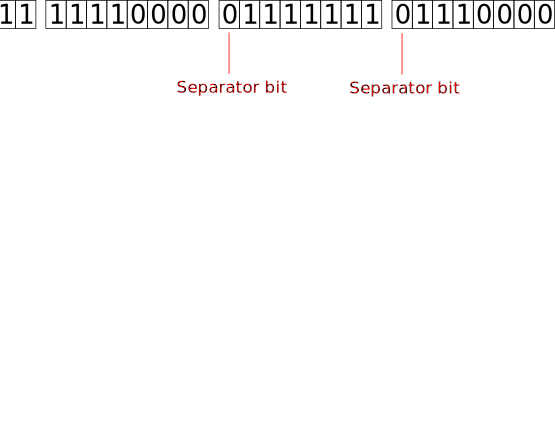
\includegraphics[width=0.8\textwidth]{figs/reply1}
	\caption{Configure reply illustration (Only first 5 bytes are shown)}
	\label{fig:JpgEpsCompare}
\end{figure}

The figure above illustrates how a reply to the configuration reply message to the message show in figure \ref{fig:config} would begin. \\\\

\noindent{}\emph{\textbf{Data message (without revolutions)}}

This section assumes that revolution counter bit depth is set to zero, meaning that revolution data is not reported by the device. See below for how the message changes when revolutions are reported.

This is the most important message -- it is used by the device to report the positions of encoders to the user.

The header of this message is a little more complex, as it carries data. Its first byte is always 0xff, its second byte is one of \{0xfc, 0xfd, 0xfe, 0xff\}, and its last byte can have many different values. When viewed as an array of 24 bits, it can be parsed thus:

\newpage{}
\begin{itemize}
\item Bits 1 to 14 -- Reserved, will always be ones.
\item Bits 15 to 20 -- Integer representing how many encoders are enabled
\item Bits 20 to 24 -- Integer representing the resolution in bits
\end{itemize}

The purpose of the reserved bits is to facilitate identification of the beginning of the message. Due to presence of separator bits (which are always zero) and maximum position resolution being 13 bits, the only situation in which 14 consecutive ones appear in data sent by the device is a message beginning.

The header is followed by a number of data bytes, which carry the positions of each enabled encoder. Each position is sent as an integer preceded by a separator bit (which will always be zero). Thus the number of bytes you should expect can be calculated after parsing the header as $ceil(\frac{(r+1)\cdot{}E}{8})$, where r is resolution in bits and E is the number of enabled encoders. The positions are sent starting in ascending order of encoder indices.

The number of encoders and resolution should fall within certain constraints. In particular, the number of enabled encoders needs to be at most 35, and the resolution needs to be between 1 and 15 bits, otherwise the 3 bytes do not form a valid data message header. Note that the header for Config reply message appears as 63 encoders running at resolution of zero bits, and thus can be differentiated from data message headers.


\textbf{Example: Data message (revolution reporting disabled)}
\begin{figure}[h]
	\centering
	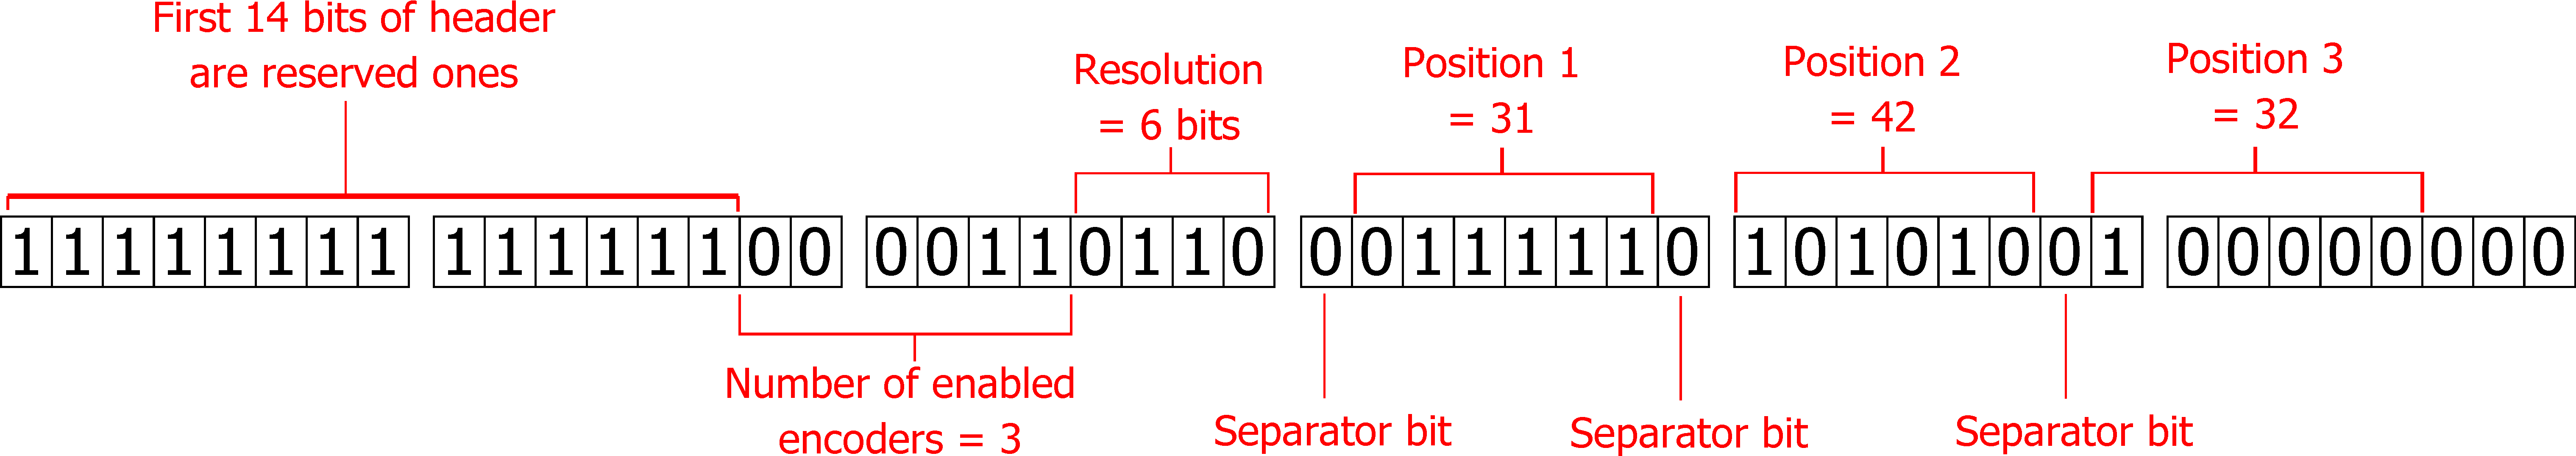
\includegraphics[width=0.9\textwidth]{figs/reply2}
	\caption{Data message illustration}

\end{figure}

Figure above shows what a data message might look like. Upon parsing the header, the user computer performs the calculation $\frac{(6+1)\cdot{}3}{8} \approx 2.6$. Rounding (always) up, we arrive at 3 -- the number of data bytes we need to receive. The last 3 bits of the third data byte do not carry any information.

Reading the positions, we see that the third encoder is in the default position, encoder number one has moved somewhat in one direction from the default and number two has moved significantly in the opposite direction.

Note that there is no indication of the actual index of the encoders -- the user needs to keep in mind which encoders they have enabled. The message above might represent the positions of encoders 1, 2 and 3. But it may also represent the positions of encoders 5, 26 and 31, if those happen to be the ones that are enabled.

\noindent{}\emph{\textbf{Data message (with revolutions reported)}}

Currently, it is not possible to differentiate between data messages with revolutions and without revolutions based just on the initial header. It is recommended for the user to note if they configured revolution counter bit depth to a nonzero value and to expect messages with revolution data if they did so.

When revolution counter bit depth is nonzero, the positions data is followed by a section of revolution data. The data section is the same as in case of data message without revolutions (see above).

The revolution data section begins with a secondary header consisting of 4 bits which encode the revolution counter bit depth used. Following the header is an array of bits in a similar format to the positions section: each revolution counter is preceded by a separation bit (always zero). Thus revolutions reporting prolongs the data message by 4+(1+R)*E bits, where R is is the revolution counter bit depth and E is the number of encoders.

The total number of bytes of the data message with revolutions is calculated as  $ceil(\frac{4+(r+R+2)\cdot{}E}{8})$, where r is the position resolution. 

Revolutions are represented as integers with offset zero. No revolutions corresponds to a value of $2^R$. This value is incremented whenever the position of the encoder in question overflows and decremented whenever it underflows.

\begin{figure}[h]
	\centering
	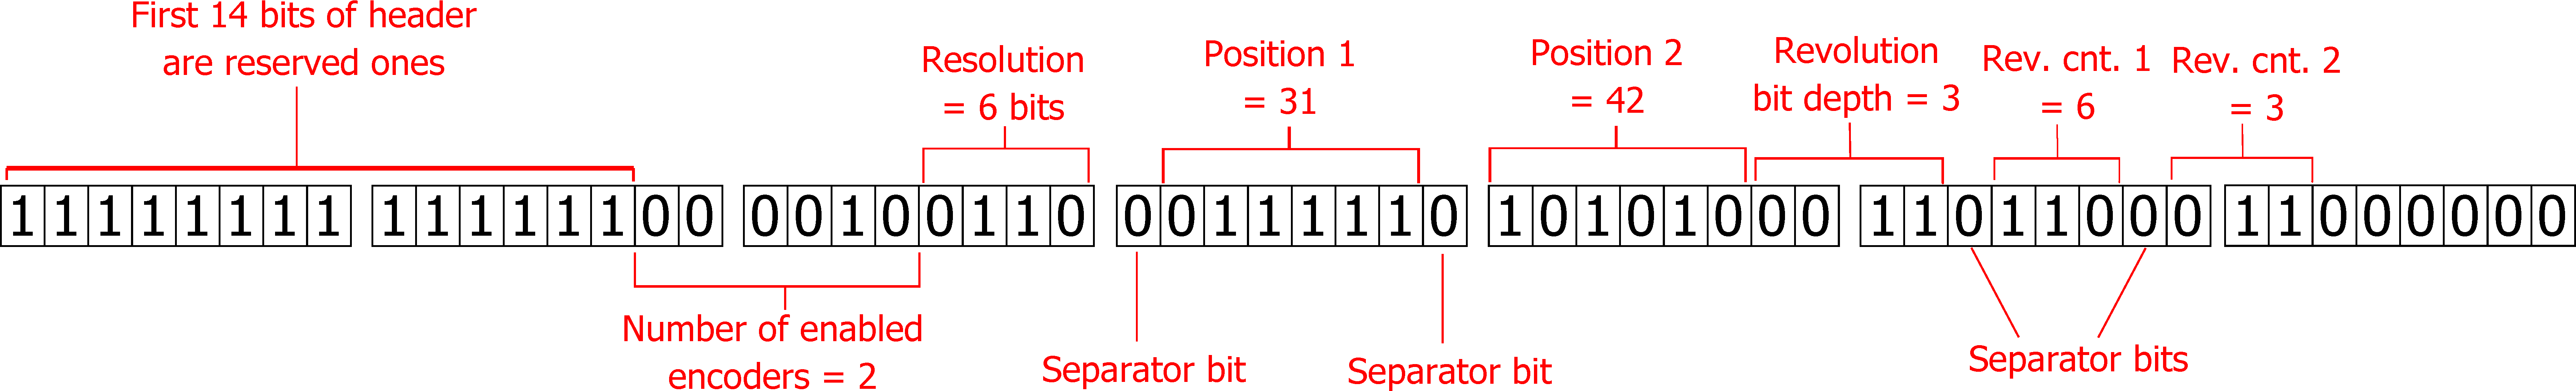
\includegraphics[width=0.9\textwidth]{figs/reply3}
	\caption{Data message illustration}
\label{fig:3}
\end{figure}

Example message is shown in figure \ref{fig:3}. Note that due to the zero offset, counter value of 6 for encoder 1 should be interpreted as that encoder performing a sum of two revolutions in one direction, while encoder 2 (counter value 3) has performed a sum of one revolution in the opposite direction. A counter value of 4 would correspond to a sum zero revolutions.

\newpage{}
\subsection{Communications demo}

\noindent{}A terminal demo script written in python is located within this repository:\\ FK\_quadrature\_decoder\textbackslash{}python\textbackslash{}CommDemo.py.

The script consists of utilities for conversion between bytes and lists of bits, as well as a function that initialises the device with desired settings and another that parses its reply. The parsing of data messages is done in a loop in the program itself.

When using the script, you may experience bytes being discarded if you set the minimum time between messages too low. In my testing, this problem appeared to be closely related to the ammount of information printed into the terminal, as well as to whether my pc was performing other intensive operations, and would lessen or disappear altogether when I redirected the script's output into a log instead of printing it to terminal. This leads me to believe that it is a fault of the computer rather than of the device; I'm guessing it's caused by a buffer overflowing somewhere. 

The script also does not (at the time of writing) check for validity of incoming data message headers.

The script was tested on windows 10 machines, using Windows Terminal\footnote{https://github.com/microsoft/terminal} (default windows cmd does not support the return codes needed to redraw multiple lines of data).

\subsection{Reconfiguring on the fly}

As a last note: the device keeps count of the positions of all  encoders at all times; not just the ones that are currently enabled for reporting. You can, therefore, begin your experiment with only some of the encoders enabled and switch to a different set of enabled encoders later -- no position reset is necessary.

\newpage{}
\section{Various technical details}

You don't need to read any further unless you're planning to modify or extend the firmware or hardware of the device.

\subsection{Cabling}

The cable used for interconnecting the pcb shield and the AMT132S encoders is 24AWG, 4-wire UTP. Wire gauge selected as only intersection that's within specs of crimp terminals on both sides.

The cable is terminated with a microclasp connector on one side and a zpd connector on the other. Since the encoders use a 18-path zpd connector (which was not available for purchase), 20-path zpd connectors cut down with a hobby knife are used instead.

\begin{figure}[h!]
	\centering
	\begin{subfigure}[b]{0.45\textwidth}
		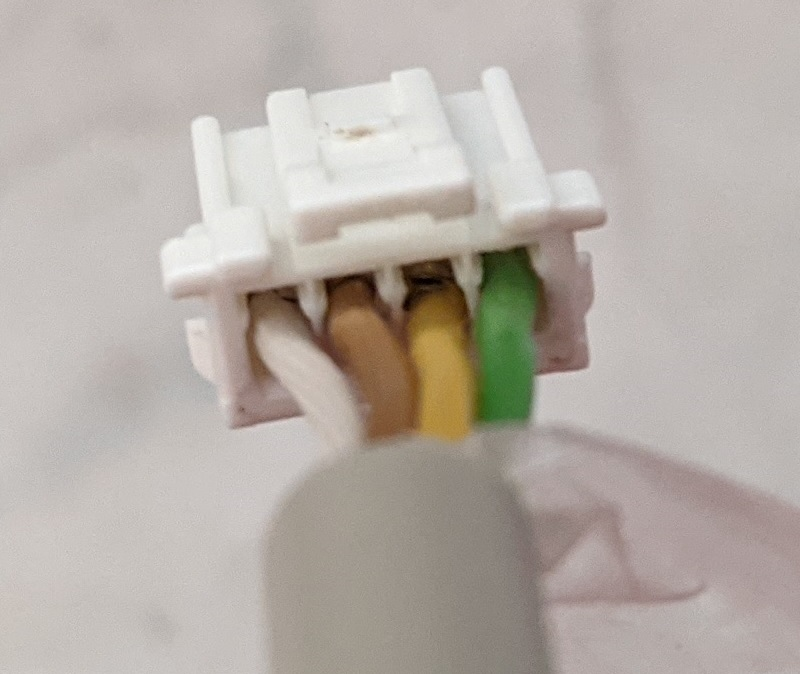
\includegraphics[width=\textwidth]{figs/conn_molex.jpg}
		\caption{Molex microclasp connector}
		\label{fig:molex}
	\end{subfigure}
	\begin{subfigure}[b]{0.45\textwidth}
		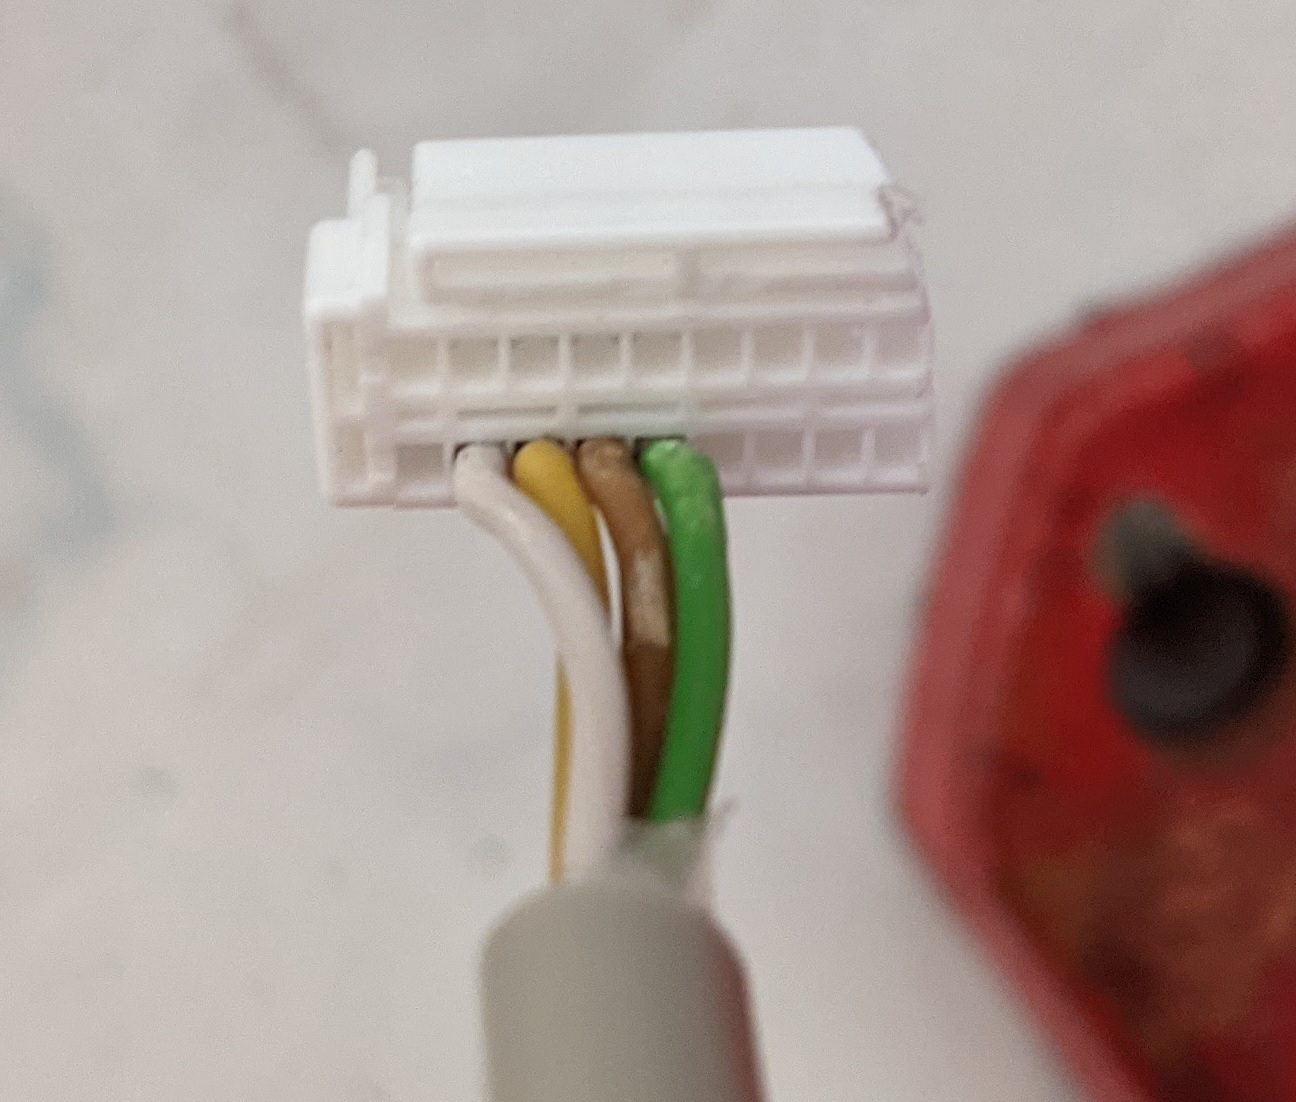
\includegraphics[width=\textwidth]{figs/conn_jst.jpg}
		\caption{JST zpd connector}
		\label{fig:jst}
	\end{subfigure}
	\caption{Cable connectors}
	\label{fig:JpgEpsCompare}
\end{figure}

The figure above shows how the wires are assigned to individual sockets of the connectors. In the photos, the wires are: 

\begin{itemize}
\item White = GND
\item Brown = Quadrature channel A
\item Yellow = +5V
\item Green = Quadrature channel B
\end{itemize}

The pairs of wires used are choosen to ensure that the quadrature channels are not twisted together.

\noindent\textbf{A note on cable assembly:} Crimping the SZPD-002T-P0.3 contacts and inserting them into the zpd housings is challenging and frustrating -- if you happen to have an idle buddhist monk at hand, this would be an ideal job to assign to them. When using the 22 AWG crimping tool I found in the lab, I had to finish the job with a pair of pliers every time, and the results were not great. Maybe try to find a 24AWG tool and/or look for a jst crimping tool\footnote{Connector datasheet http://www.farnell.com/datasheets/2261947.pdf lists some industrial-looking crimping machines.}.


\subsection{PCB bug (turning off & FT232)}
\label{hwbug}

There is an error in the the pcb design, necessitating a specific order in which the power and usb cables can be unplugged from the device when turning it off, as described in \ref{turnoff}. 

To fix this issue, 3 components need to be added to the pcb - two resistors (80k, 4k) and a generic NPN transistor. Those components, as well as their placement in the circuit, have been added to the kicad schematic of the PCB (see blue box next to the FT232 symbol).

If you don't want to add the components to the PCB itself, you can still solve the problem (we have solved it this way). To solder the components, you will need to make use of pads originally intended for the R1 resistor (which is now left unpopulated, see schematic). The third needed solder point is the 5V power rail. This is easily accesible via the unpopulated J37 2x4 connector, next to the usb connector.

\subsection{Firmware structure}

The fpga firmware is provided as a quartus II project. The design is split into several entities:

\subsubsection{FK quadrature decoder}

This is the top-level entity, dealing with interconnections between all other entities and with GPIO mappings.

\subsubsection{Uart TX / Uart RX}

Simple entities implementing uart transmitter and receiver. Input/output is a single byte, buffering etc. is handled in other entities.

\subsubsection{Uart out manager}

This entity takes a series of bytes and feeds them in order into the Uart TX entity, which transmits them. The bytes are provided to the manager either by the Watcher or by the Boss entity, with Boss entity having precedence.

\subsubsection{Boss}

This entity receives and interprets communication from the user into the fpga, and is also responsible for changing configuration of the Watcher entity when a config message is received from the user. Additionally, it also creates the config reply message and passes it to Uart out manager.

\subsubsection{Watcher}

This entity is responsible for periodically sampling all connected quadrature encoders and assembling data messages (which it passes to uart out manager). It holds within itself an array of 35 Quadrature Decoder Pb entities. The parameters of the data message (such as resolution or which encoders are reported) as well as the frequency with which data messages are created is governed by inputs driven by the Boss entity.

\subsubsection{Quadrature Decoder Pb}

This is a simple entity handling the decoding of quadrature signals for a single encoder. It takes in the two quadrature signals and outputs position and number of resolutions (to the Watcher entity).







\end{document}

